\documentclass[tikz, border=10pt]{standalone}
\usetikzlibrary{angles, quotes}

\usetikzlibrary{calc}
\begin{document}
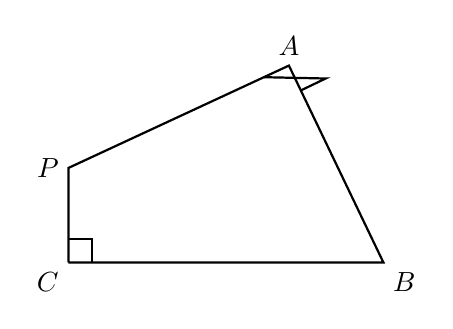
\begin{tikzpicture}[scale=1]
  % Coordinates
  \coordinate (C) at (0,0);
  \coordinate (B) at (4,0);
  \coordinate (A) at (2.8,2.5);
  \coordinate (P) at (0,1.2);

  % Polygon edges
  \draw[thick] (C) -- (B) -- (A) -- (P) -- (C);

  % Right angle marks
  \draw[thick] (0.3,0) -- (0.3,0.3) -- (0,0.3);
  \draw[thick]
    ($(A)!0.35cm!(B)$) -- ($($(A)!0.35cm!(B)$)!0.35cm!90:(B)$) -- ($(A)!0.35cm!(P)$);

  % Labels
  \node[above] at (A) {$A$};
  \node[below right] at (B) {$B$};
  \node[below left] at (C) {$C$};
  \node[left] at (P) {$P$};
\end{tikzpicture}
\end{document}
